% Apresentação de Defesa de TCC - Daniel Cavalli (VERSÃO 4 - REVISADA)
% Instituto de Economia - UFRJ
% 2025

\documentclass[10pt,aspectratio=169]{beamer}

% Pacotes essenciais
\usepackage[brazilian]{babel}
\usepackage[utf8]{inputenc}
\usepackage[T1]{fontenc}
\usepackage{amsmath,amssymb}
\usepackage{graphicx}
\usepackage{booktabs}
\usepackage{multirow}
\usepackage{tikz}
\usetikzlibrary{positioning}
\usepackage{pgfplots}
\pgfplotsset{compat=1.17}

% Configuração do tema
\usetheme{Boadilla}
\usecolortheme{default}
\setbeamertemplate{navigation symbols}{}
\setbeamertemplate{footline}[frame number]

% Remove sombras e elementos decorativos
\setbeamertemplate{blocks}[rounded][shadow=false]
\setbeamertemplate{title page}[default][colsep=-4bp,rounded=false,shadow=false]
\setbeamertemplate{frametitle}[default][colsep=-2bp,rounded=false,shadow=false,center]

% Cores personalizadas UFRJ
\definecolor{ufrjblue}{RGB}{0,53,96}
\definecolor{ufrjgreen}{RGB}{0,128,0}
\definecolor{ufrjlightblue}{RGB}{51,102,153}
\definecolor{ufrjgray}{RGB}{100,100,100}

% Aplicação sutil das cores
\setbeamercolor{structure}{fg=ufrjblue}
\setbeamercolor{frametitle}{bg=white,fg=ufrjblue}
\setbeamercolor{title}{fg=ufrjblue}
\setbeamercolor{block title}{bg=ufrjlightblue,fg=white}
\setbeamercolor{block body}{bg=ufrjlightblue!10}
\setbeamercolor{block title alerted}{bg=red!90,fg=white}
\setbeamercolor{block body alerted}{bg=red!10}

% Configuração de itemize/enumerate
\setbeamercolor{itemize item}{fg=ufrjblue}
\setbeamercolor{itemize subitem}{fg=ufrjlightblue}
\setbeamercolor{enumerate item}{fg=ufrjblue}

% Configurações de fonte
\usefonttheme{professionalfonts}
\setbeamerfont{title}{size=\Large,series=\bfseries}
\setbeamerfont{frametitle}{size=\large,series=\bfseries}
\setbeamerfont{block title}{size=\normalsize,series=\bfseries}

% Configurações adicionais para design limpo
\setbeamertemplate{itemize items}[circle]
\setbeamertemplate{enumerate items}[default]
\setbeamertemplate{section in toc}[circle]

% Remove linhas de separação
\setbeamertemplate{headline}{}
\setbeamertemplate{footline}{
    \leavevmode%
    \hbox{%
    \begin{beamercolorbox}[wd=.333333\paperwidth,ht=2.25ex,dp=1ex,center]{author in head/foot}%
        \usebeamerfont{author in head/foot}\insertshortauthor
    \end{beamercolorbox}%
    \begin{beamercolorbox}[wd=.333333\paperwidth,ht=2.25ex,dp=1ex,center]{title in head/foot}%
        \usebeamerfont{title in head/foot}\insertshorttitle
    \end{beamercolorbox}%
    \begin{beamercolorbox}[wd=.333333\paperwidth,ht=2.25ex,dp=1ex,right]{date in head/foot}%
        \usebeamerfont{date in head/foot}\insertshortdate{}\hspace*{2em}
        \insertframenumber{} / \inserttotalframenumber\hspace*{2ex} 
    \end{beamercolorbox}}%
    \vskip0pt%
}

% Ajuste de margens para mais espaço
\setbeamersize{text margin left=1em,text margin right=1em}

% Informações do documento
\title[Estações Meteorológicas e Produtividade Agrícola]{Impacto de Estações Meteorológicas na Produtividade Agrícola: \\ Uma Aplicação de Diferenças em Diferenças com Tratamento Escalonado}

\author[Daniel Cavalli]{Daniel Cavalli \\ \small Orientador: Prof. Romero Rocha}

\institute[IE-UFRJ]{
  Instituto de Economia\\
  Universidade Federal do Rio de Janeiro
}

\date{2025}

% Importa valores automaticamente gerados
% Arquivo gerado automaticamente por generate_latex_values.r
% Última atualização: 2025-09-07

% Valores do teste placebo aleatório
\newcommand{\placebotruatt}{0.082}
\newcommand{\placebopvalue}{< 0,001}
\newcommand{\placebolower}{-0.037}
\newcommand{\placeboupper}{0.033}
\newcommand{\placebonsims}{50}
\newcommand{\placebomean}{-0.002}

% Valores formatados para texto
\newcommand{\placebotruattpct}{8.2\%}
\newcommand{\placebopvaluepct}{< 1\%}

% Valores do modelo principal
\newcommand{\mainatt}{0.082}
\newcommand{\mainse}{0.032}
\newcommand{\mainattpct}{8.2\%}

% Valores da análise de sensibilidade temporal
% Completo (2003-2023)
\newcommand{\sensfullatt}{0.126}
\newcommand{\sensfullse}{0.029}
\newcommand{\sensfulllower}{0.070}
\newcommand{\sensfullupper}{0.182}
\newcommand{\sensfulln}{7371}
% Excluindo Início (2006-2023)
\newcommand{\sensnostartatt}{0.130}
\newcommand{\sensnostartse}{0.031}
\newcommand{\sensnostartlower}{0.069}
\newcommand{\sensnostartupper}{0.191}
\newcommand{\sensnostartn}{6318}
% Excluindo Final (2003-2019)
\newcommand{\sensnoendatt}{0.117}
\newcommand{\sensnoendse}{0.027}
\newcommand{\sensnoendlower}{0.065}
\newcommand{\sensnoendupper}{0.170}
\newcommand{\sensnoendn}{5967}
% Excluindo COVID (2003-2019)
\newcommand{\sensnocovidatt}{0.117}
\newcommand{\sensnocovidse}{0.026}
\newcommand{\sensnocovidlower}{0.066}
\newcommand{\sensnocovidupper}{0.169}
\newcommand{\sensnocovidn}{5967}
% Pré-COVID (2003-2019)
\newcommand{\sensprecovidatt}{0.117}
\newcommand{\sensprecovidse}{0.025}
\newcommand{\sensprecovidlower}{0.068}
\newcommand{\sensprecovidupper}{0.167}
\newcommand{\sensprecovidn}{5967}


% Início do documento
\begin{document}

% Slide título
\begin{frame}
\titlepage
\end{frame}

% Sumário
\begin{frame}{Roteiro}
\tableofcontents
\end{frame}

% ===== SEÇÃO 1: MOTIVAÇÃO E PROBLEMA =====
\section{Motivação e Problema de Pesquisa}

\begin{frame}{Contexto}
\begin{columns}
\column{0.5\textwidth}
\textbf{Desafio da Agricultura:}
\begin{itemize}
    \item Crescente variabilidade climática
    \item Necessidade de aumento de produtividade
    \item Informação como insumo produtivo
\end{itemize}

\vspace{0.5cm}
\textbf{Lacuna na Literatura:}
\begin{itemize}
    \item Estudos predominantemente descritivos
    \item Ausência de evidências causais
    \item Falta quantificação econômica rigorosa
\end{itemize}

\column{0.5\textwidth}
\begin{block}{Oportunidade}
Instalação escalonada de estações meteorológicas (2000-2019) cria experimento natural
\end{block}

\vspace{0.3cm}
\begin{alertblock}{Questão Central}
Qual o impacto causal da instalação de estações meteorológicas sobre o PIB agropecuário?
\end{alertblock}
\end{columns}
\end{frame}

\begin{frame}{Mecanismo Causal}
\begin{figure}
\centering
\begin{tikzpicture}[scale=0.9, every node/.style={font=\small}]
% Caixas
\node[draw, rectangle, minimum width=2.5cm, minimum height=0.8cm, align=center] (est) at (0,0) {Estação\\Meteorológica};
\node[draw, rectangle, minimum width=2.5cm, minimum height=0.8cm, align=center] (dados) at (4,0) {Dados\\Climáticos};
\node[draw, rectangle, minimum width=2.5cm, minimum height=0.8cm, align=center] (dec) at (8,0) {Decisões\\Otimizadas};
\node[draw, rectangle, minimum width=2.5cm, minimum height=0.8cm, align=center] (pib) at (12,0) {$\uparrow$ PIB\\Agropecuário};

% Setas
\draw[->, thick] (est) -- (dados);
\draw[->, thick] (dados) -- (dec);
\draw[->, thick] (dec) -- (pib);

% Exemplos abaixo
\node[below of=dados, node distance=0.8cm, align=center, font=\tiny] {Temperatura\\Precipitação\\Eventos extremos};
\node[below of=dec, node distance=0.8cm, align=center, font=\tiny] {Plantio/Colheita\\Irrigação\\Defensivos};
\end{tikzpicture}
\end{figure}

\vspace{0.3cm}
\textbf{Literatura identifica três dimensões} (Mavi e Tupper, 2004):
\begin{enumerate}
    \item Planejamento estratégico
    \item Decisões táticas
    \item Construção de resiliência
\end{enumerate}

\textbf{+ Canal indireto:} Modelos de simulação (ex: DSSAT-CANEGRO)
\end{frame}

% ===== SEÇÃO 2: ESTRATÉGIA EMPÍRICA =====
\section{Estratégia Empírica}

\begin{frame}{Dados e Definições}
\begin{columns}
\column{0.6\textwidth}
\textbf{Amostra:}
\begin{itemize}
    \item 490 microrregiões brasileiras
    \item Critério: produtoras de cana-de-açúcar
    \item Período: 2003-2023 (21 anos)
    \item 10.290 observações
\end{itemize}

\vspace{0.3cm}
\textbf{Definições:}
\begin{itemize}
    \item \textbf{Tratamento}: Instalação da primeira estação
    \item \textbf{Outcome}: $Y_{it} = \ln(1 + \text{PIB\_Agro}_{it})$
    \item \textbf{Grupo}: $G_i$ = ano da primeira estação
\end{itemize}

\column{0.4\textwidth}
\begin{figure}
\centering
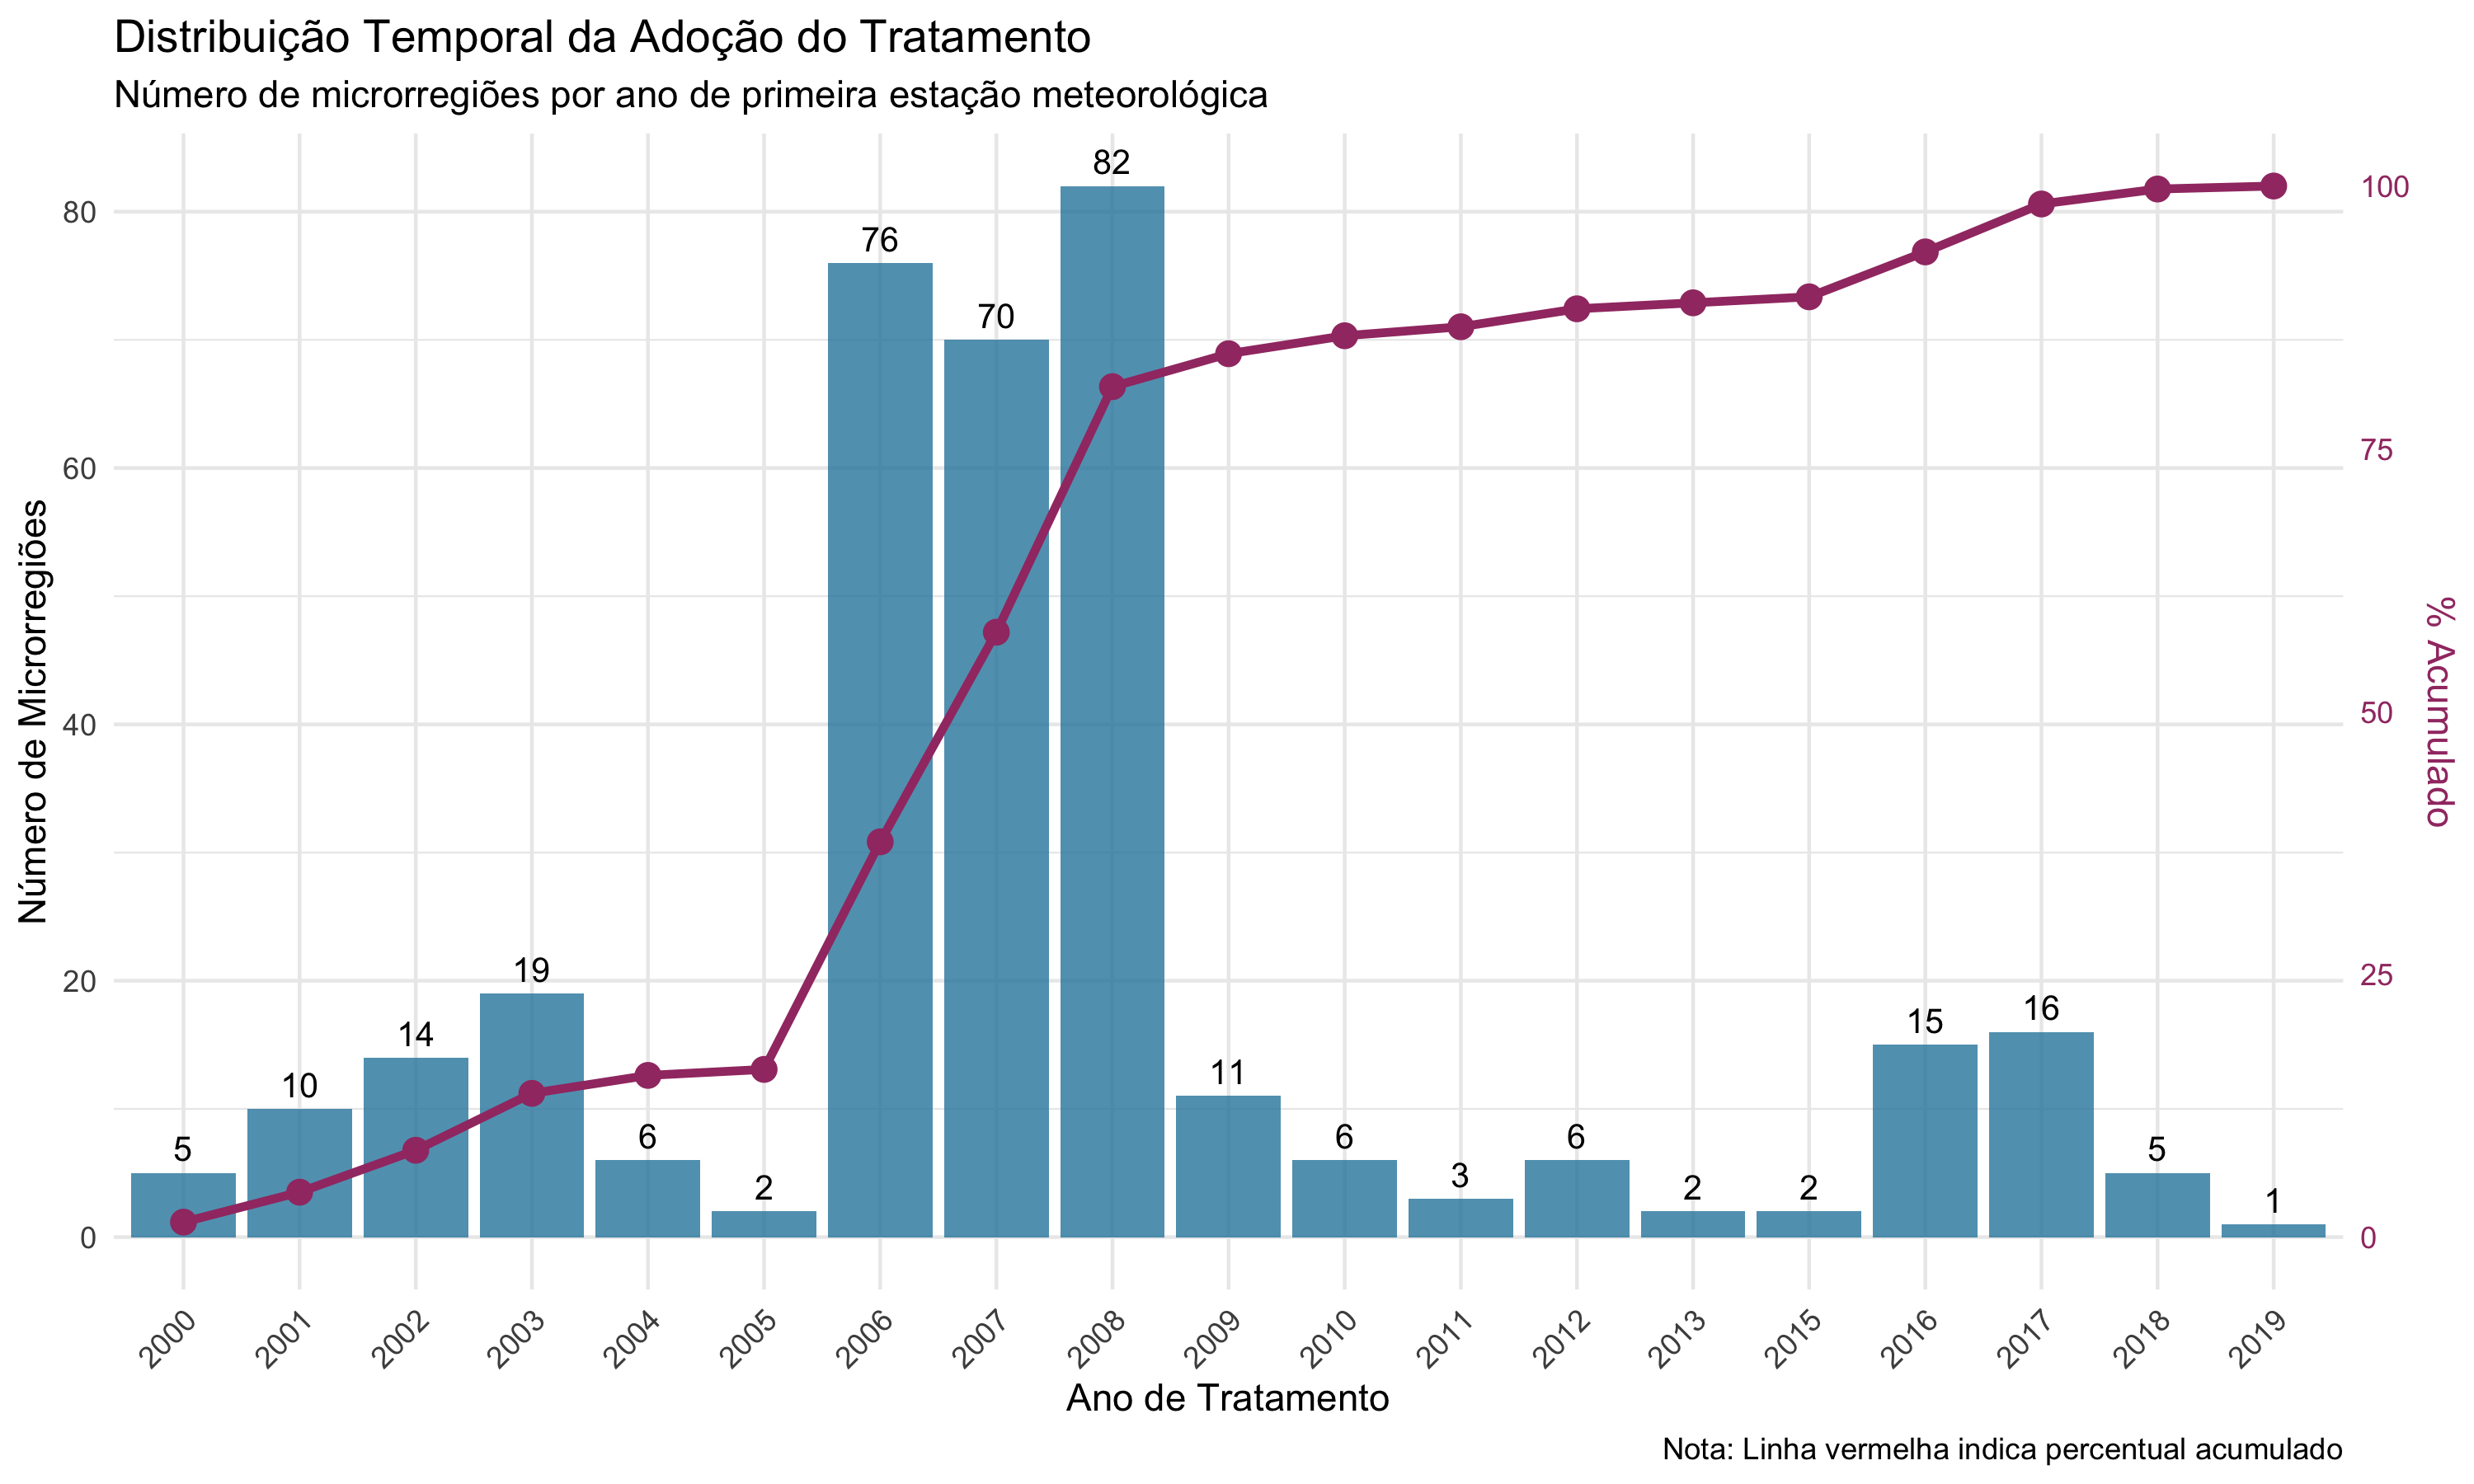
\includegraphics[width=\textwidth]{../../../data/outputs/descriptive_analysis/distribuicao_temporal_tratamento.png}
\caption{Distribuição temporal do tratamento}
\end{figure}

\begin{block}{Status}
351 microrregiões tratadas (71,6\%)
\end{block}
\end{columns}
\end{frame}

\begin{frame}{O Problema do Tratamento Escalonado}
\begin{columns}
\column{0.6\textwidth}
\textbf{TWFE Tradicional:}
$$Y_{it} = \alpha_i + \lambda_t + \beta D_{it} + \epsilon_{it}$$

\textbf{Problemas Identificados:}
\begin{itemize}
    \item Usa já tratados como controle
    \item Pesos potencialmente negativos
    \item Viés com efeitos heterogêneos
\end{itemize}

\vspace{0.3cm}
Goodman-Bacon (2021), Sun e Abraham (2021)

\column{0.4\textwidth}
\begin{figure}
\centering
\begin{tikzpicture}[scale=0.8]
\draw[->] (0,0) -- (5,0) node[right] {$t$};
\draw[->] (0,0) -- (0,3.5) node[above] {Unidades};

% Grupos
\draw[thick,blue] (0.5,0.5) -- (1.5,0.5);
\draw[thick,blue,dashed] (1.5,0.5) -- (1.5,0.8);
\draw[thick,blue] (1.5,0.8) -- (4.5,0.8);

\draw[thick,red] (0.5,1.5) -- (2.5,1.5);
\draw[thick,red,dashed] (2.5,1.5) -- (2.5,1.8);
\draw[thick,red] (2.5,1.8) -- (4.5,1.8);

\draw[thick,green] (0.5,2.5) -- (4.5,2.5);

% Problema
\draw[<->, orange, thick] (1.5,0.9) -- (2.5,1.4);
\node[orange, right, align=center] at (2.7,1.15) {\tiny Comparação\\\tiny problemática};
\end{tikzpicture}
\caption{Comparações inadequadas no TWFE}
\end{figure}
\end{columns}
\end{frame}

% ===== SEÇÃO 3: METODOLOGIA =====
\section{Metodologia: Callaway e Sant'Anna (2021)}

\begin{frame}{Solução: DiD com Múltiplos Períodos}
\textbf{Abordagem em 3 etapas:}

\vspace{0.3cm}
\begin{enumerate}
    \item \textbf{Estimação Desagregada}
    \begin{itemize}
        \item ATT(g,t): efeito para grupo $g$ no tempo $t$
        \item Comparação apenas com "not-yet-treated"
    \end{itemize}
    
    \vspace{0.3cm}
    \item \textbf{Agregação}
    \begin{itemize}
        \item Overall ATT: $\theta_{sel}^O = \sum_g \theta_{sel}(g) \cdot P(G=g|G \leq T)$
        \item Event study: $\theta_{es}^{bal}(e)$ para tempo relativo $e$
    \end{itemize}
    
    \vspace{0.3cm}
    \item \textbf{Inferência}
    \begin{itemize}
        \item Bootstrap multiplicativo (1.000 replicações)
        \item Clustering ao nível da microrregião
    \end{itemize}
\end{enumerate}

\vspace{0.3cm}
\textbf{Estimador:} Doubly Robust (DR) - consistente se outcome regression OU propensity score correto
\end{frame}

\begin{frame}{Validação dos Pressupostos}
\begin{columns}
\column{0.5\textwidth}
\textbf{1. Tendências Paralelas}
\begin{itemize}
    \item Visual: Event study pré-tratamento
    \item Formal: Teste F por coorte
    \item Resultado: F = 1,136 (p = 0,322)
\end{itemize}

\vspace{0.3cm}
\textbf{2. No Anticipation}
\begin{itemize}
    \item Efeitos apenas após instalação física
    \item Se violado: estimativas conservadoras
\end{itemize}

\column{0.5\textwidth}
\textbf{3. Tratamento Irreversível}
\begin{itemize}
    \item Estações permanecem ativas
    \item Consistente com dados observados
\end{itemize}

\vspace{0.3cm}
\textbf{4. Overlap}
\begin{itemize}
    \item Características sobrepostas
    \item Garantido pela seleção da amostra
\end{itemize}
\end{columns}

\vspace{0.5cm}
\begin{alertblock}{Validação}
Todos os pressupostos testados e validados empiricamente
\end{alertblock}
\end{frame}

% ===== SEÇÃO 4: RESULTADOS PRINCIPAIS =====
\section{Resultados}

\begin{frame}{Efeito Médio do Tratamento (ATT)}
\begin{center}
\huge
\textbf{ATT = \mainatt}\\
\large
\textbf{(Aumento de \mainattpct{} no PIB agropecuário)}\\
\normalsize
\vspace{0.5cm}
Erro Padrão = \mainse\\
IC 95\%: [1,9\%; 14,5\%]\\
p-valor = 0,0103
\end{center}

\vspace{0.5cm}

\begin{columns}
\column{0.5\textwidth}
\begin{block}{Interpretação}
Equivale a mais de 2 anos de crescimento típico do setor (3-4\% a.a.)
\end{block}

\column{0.5\textwidth}
\begin{block}{Robustez}
\begin{itemize}
    \item DR: 8,2\% (p = 0,010)
    \item IPW: 9,4\% (p = 0,003)
    \item REG: 6,6\% (p = 0,030)
\end{itemize}
\end{block}
\end{columns}
\end{frame}

\begin{frame}{Event Study: Dinâmica Temporal}
\begin{figure}
\centering
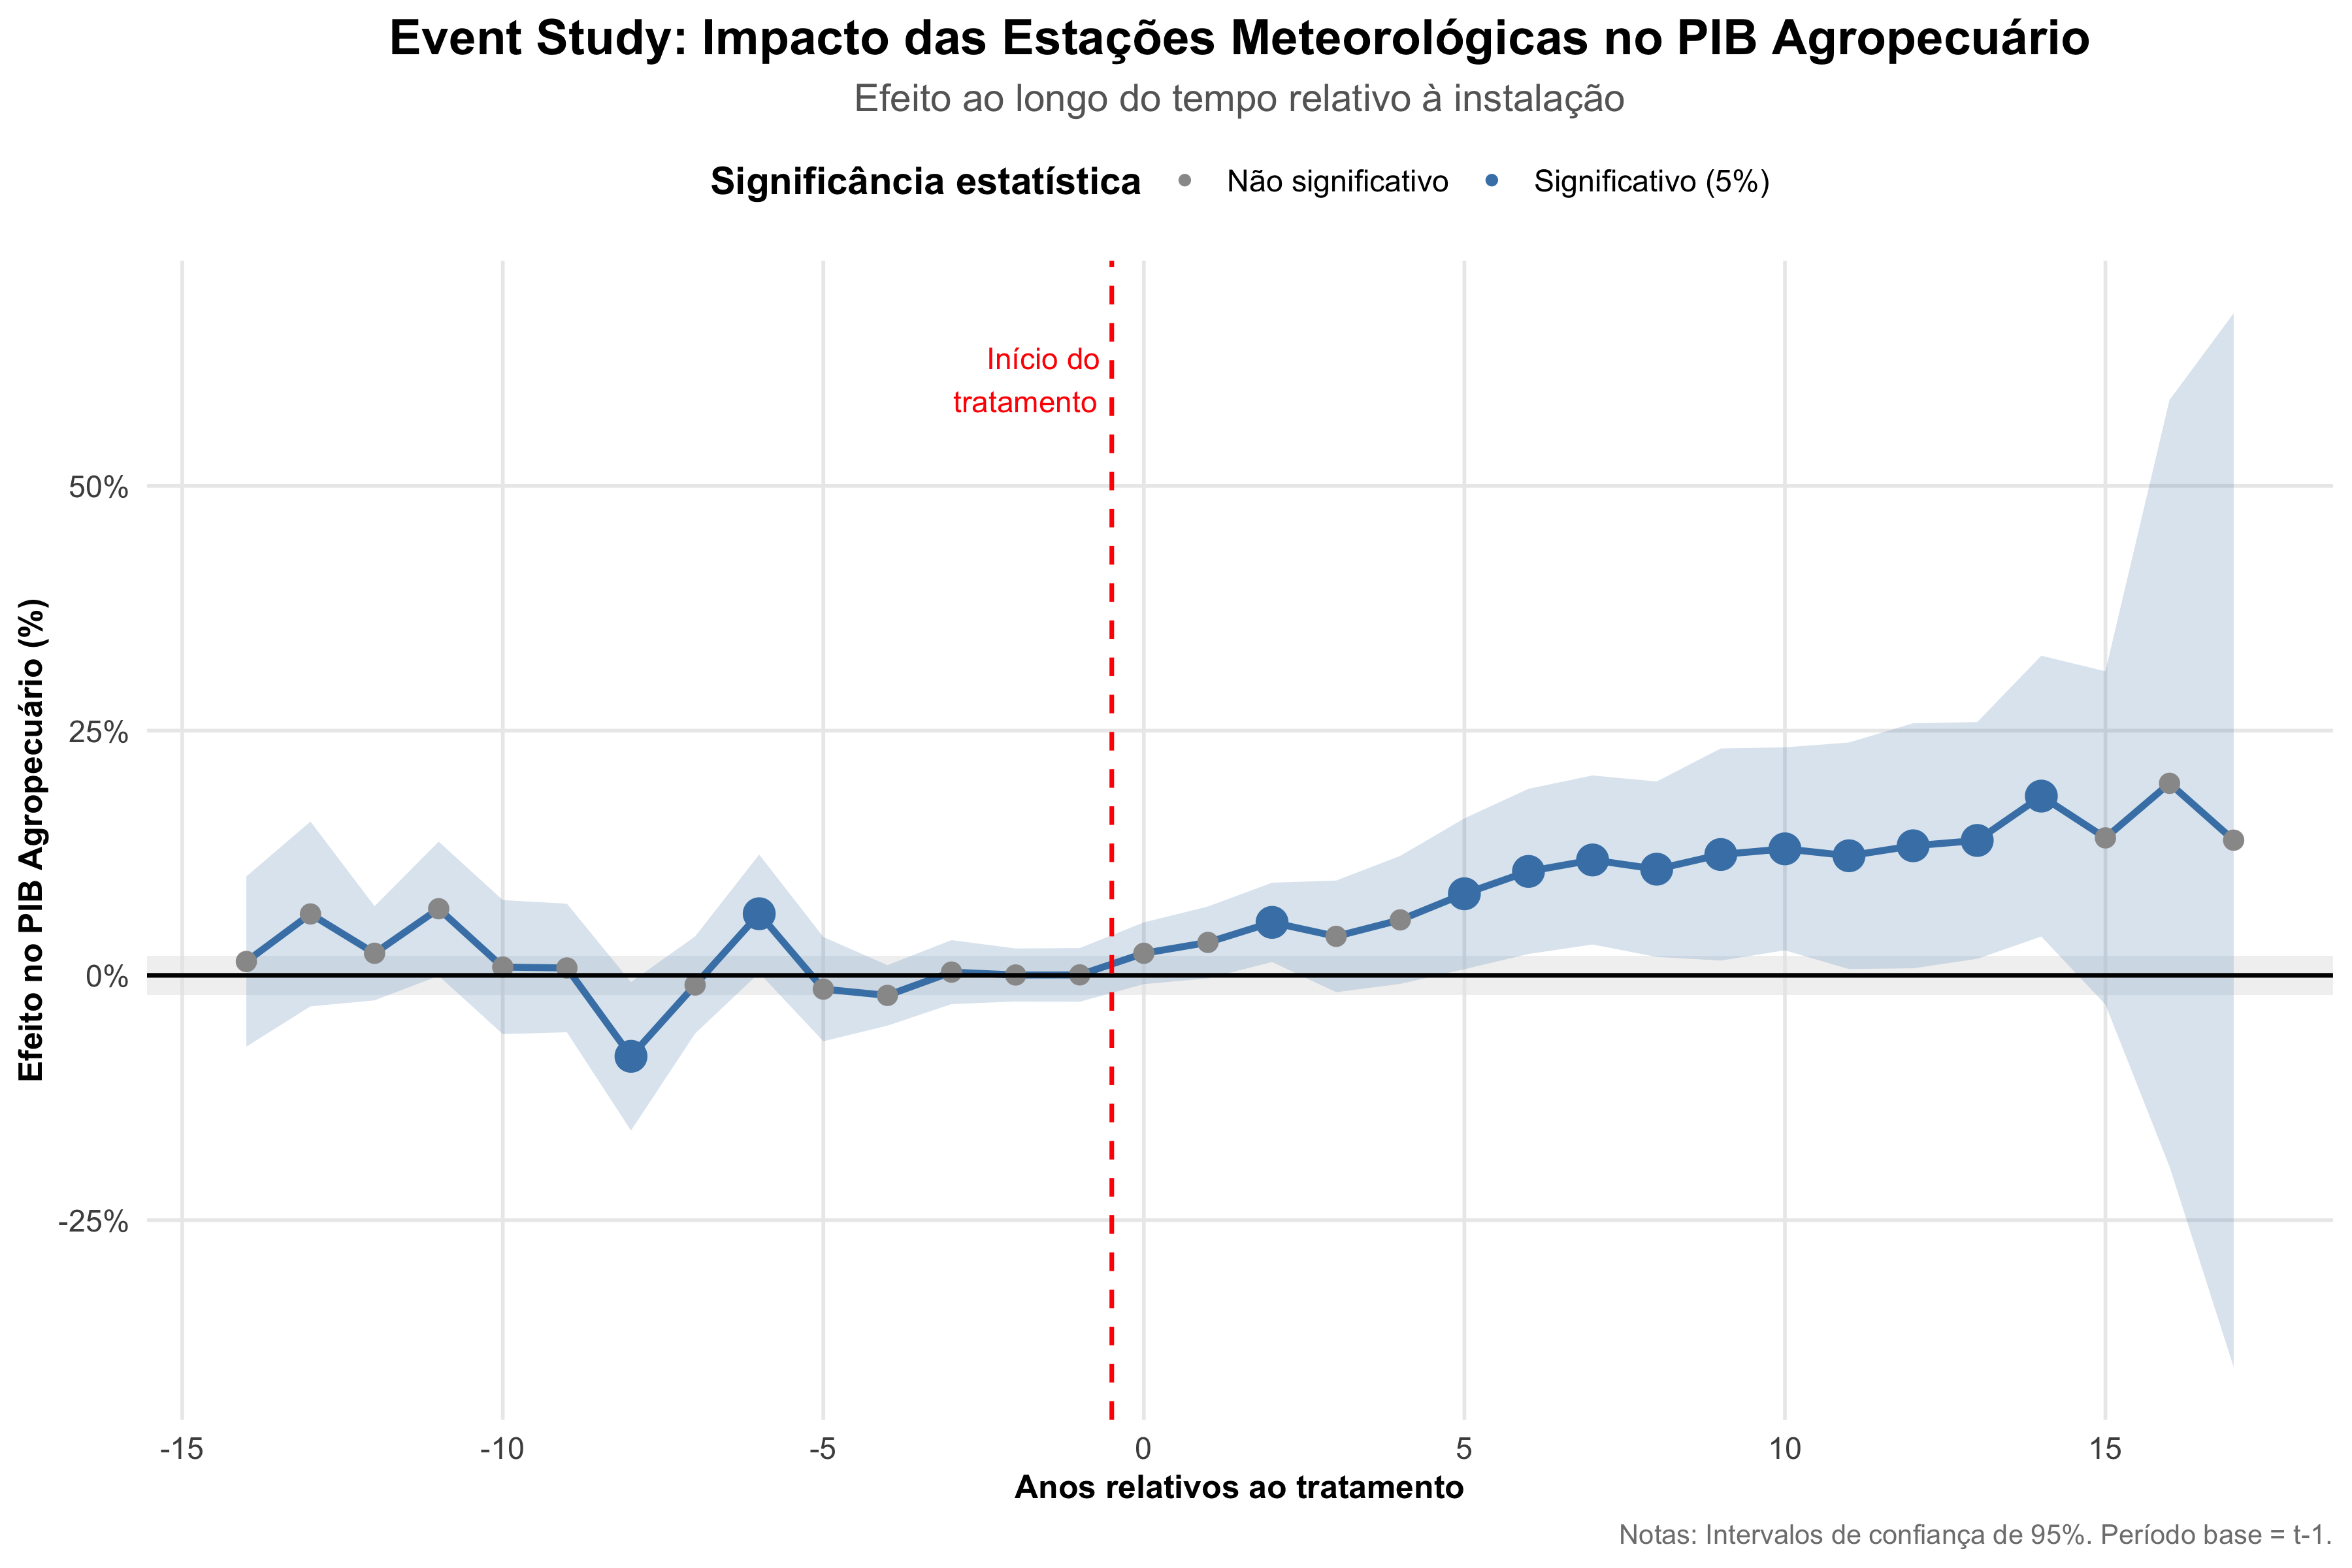
\includegraphics[width=0.85\textwidth]{../../../data/outputs/presentation/event_study_enhanced.png}
\end{figure}

\textbf{Evidências-chave:}
\begin{itemize}
    \item Pré-tratamento: ausência de tendências diferenciadas (validação)
    \item Pós-tratamento: efeitos emergem gradualmente
    \item Estabilização em ~10\% após 5 anos (processo de aprendizado)
\end{itemize}
\end{frame}

% ===== SEÇÃO 5: VALIDAÇÃO CAUSAL =====
\section{Testes de Robustez}

\begin{frame}{Teste de Randomização de Monte Carlo}
\begin{columns}
\column{0.5\textwidth}
\textbf{Procedimento:}
\begin{enumerate}
    \item 5.000 simulações independentes
    \item Randomizar tratamento:
    \begin{itemize}
        \item Quais unidades
        \item Quando tratadas
    \end{itemize}
    \item Estimar ATT para cada simulação
    \item Construir distribuição empírica
\end{enumerate}

\vspace{0.3cm}
\textbf{P-valor empírico:}
$$\hat{p} = \frac{1 + \sum \mathbb{1}\{|ATT^s| \geq |ATT^{obs}|\}}{5001}$$

\column{0.5\textwidth}
\begin{figure}
\centering
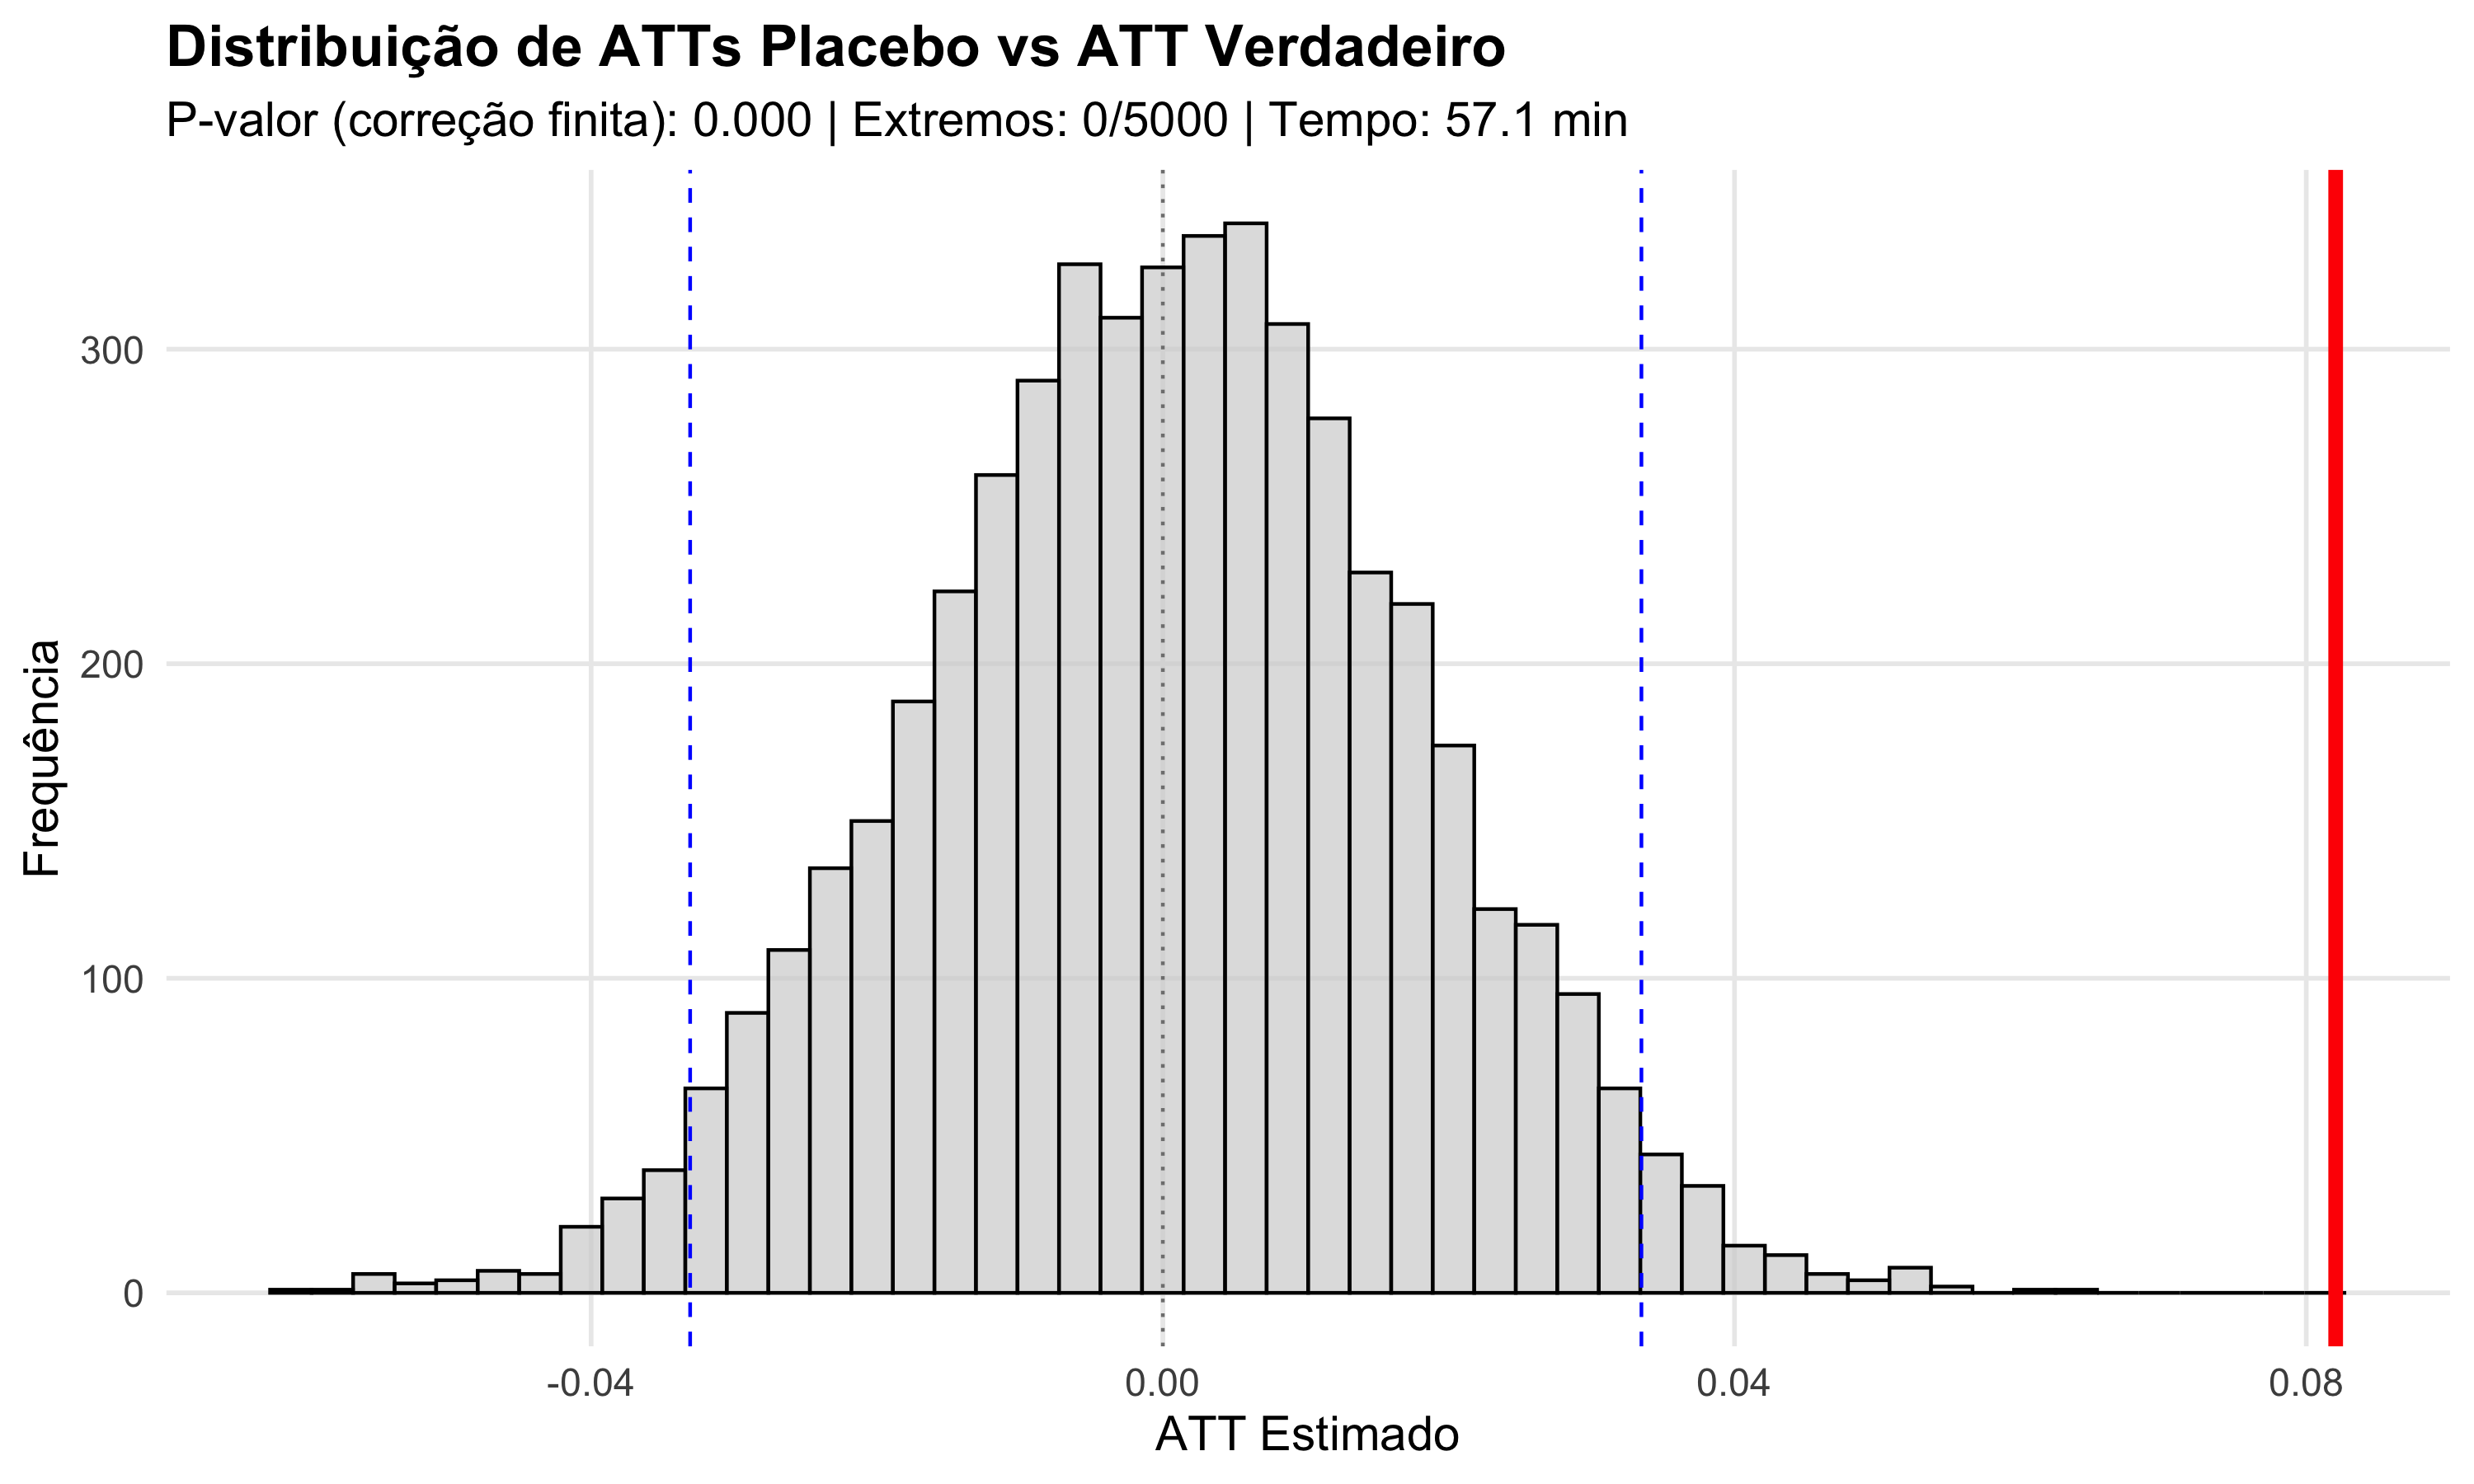
\includegraphics[width=\textwidth]{../../../data/outputs/placebo_distribution.png}
\end{figure}

\begin{alertblock}{Resultado}
P-valor < 0,001\\
Menos de 0,1\% das simulações com efeito similar
\end{alertblock}
\end{columns}
\end{frame}

\begin{frame}{Testes Placebo e Sensibilidade}
\begin{columns}
\column{0.5\textwidth}
\textbf{1. PIB Não-Agropecuário}
\begin{itemize}
    \item ATT = 0,015 (p = 0,427)
    \item Não significativo
    \item Confirma especificidade setorial
\end{itemize}

\vspace{0.3cm}
\textbf{2. Atribuição Aleatória}
\begin{itemize}
    \item 50\% tratadas em 2015
    \item ATT = -0,024 (p = 0,485)
    \item Modelo não gera efeitos espúrios
\end{itemize}

\column{0.5\textwidth}
\textbf{3. Sensibilidade Temporal}
\begin{itemize}
    \item Completo: 12,6\%***
    \item Sem COVID: 11,7\%***
    \item Sem início: 13,0\%***
\end{itemize}

\vspace{0.3cm}
\textbf{4. Grupo de Controle}
\begin{itemize}
    \item Not-yet-treated: 8,2\%***
    \item Never-treated: 8,0\%**
\end{itemize}
\end{columns}

\vspace{0.5cm}
\begin{center}
\textbf{Conclusão: Efeito causal robusto e específico à agricultura}
\end{center}
\end{frame}

\begin{frame}{Síntese da Robustez}
\begin{figure}
\centering
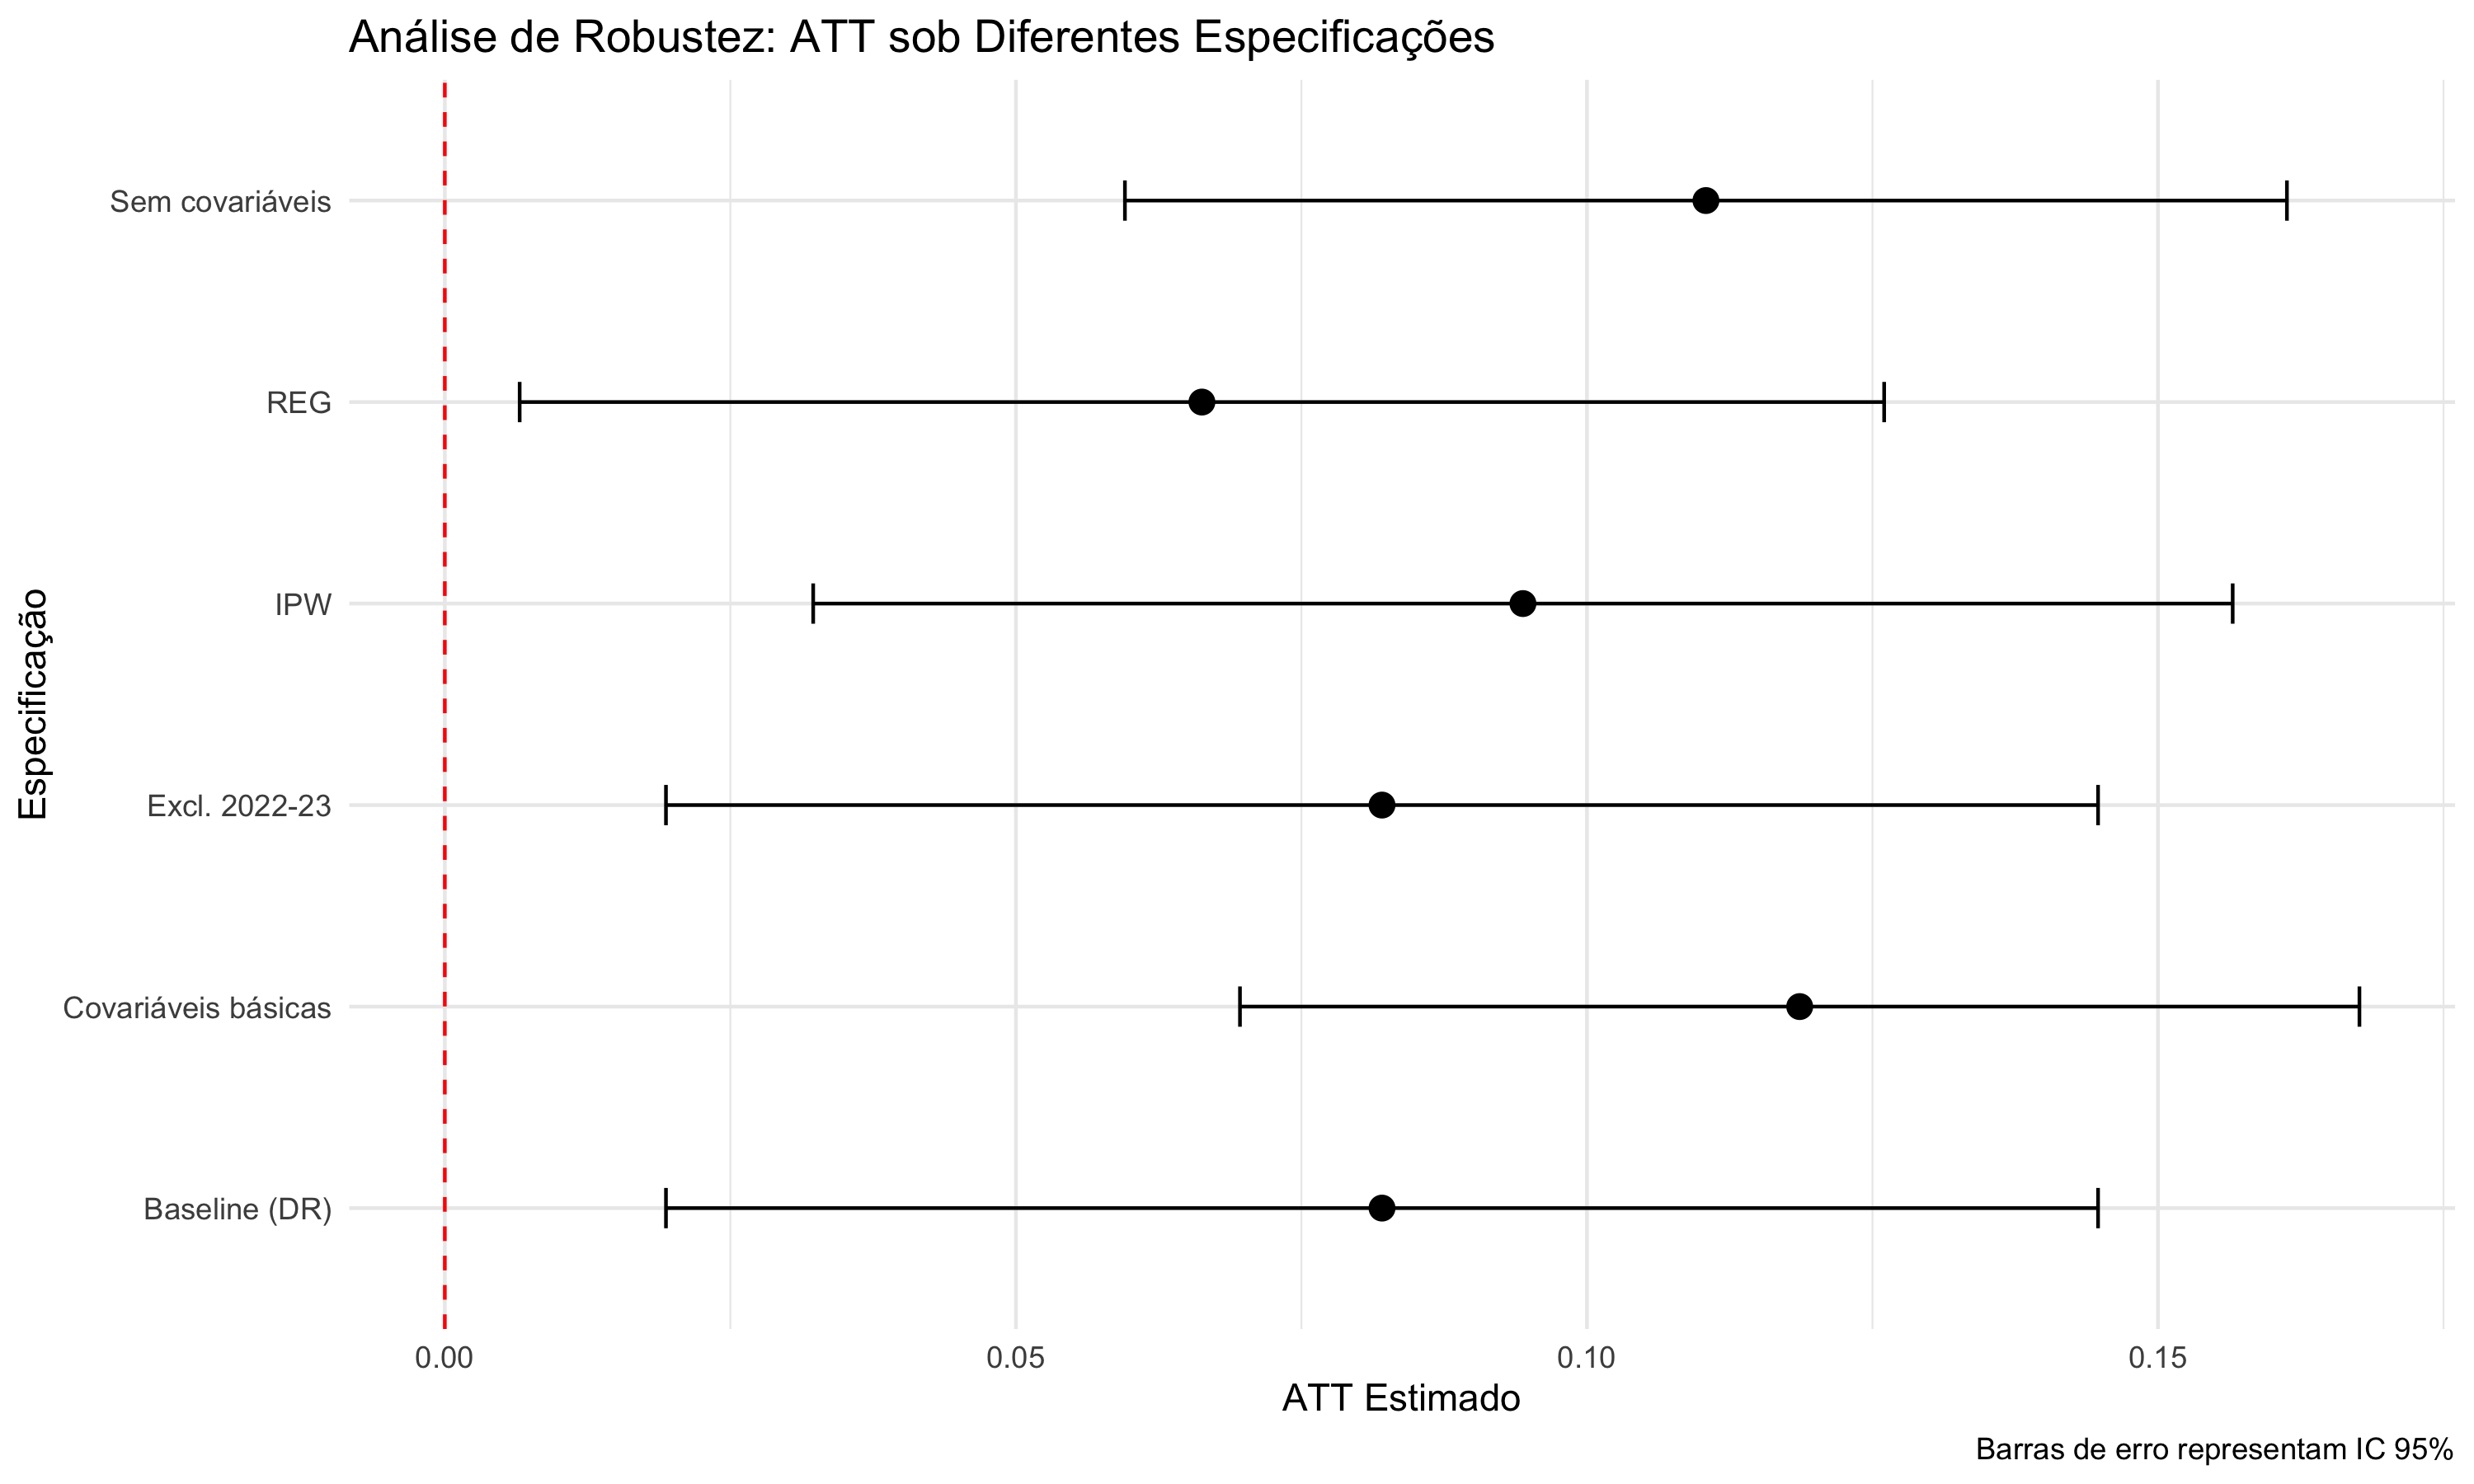
\includegraphics[width=0.9\textwidth]{../../../data/outputs/robustness_plot.png}
\end{figure}

\textbf{Mensagem central:} Efeito consistente entre 6-13\% em todas as especificações
\end{frame}

% ===== SEÇÃO 6: IMPLICAÇÕES =====
\section{Implicações Econômicas e de Política}

\begin{frame}{Magnitude Econômica}
\begin{columns}
\column{0.6\textwidth}
\textbf{Contextualização:}
\begin{itemize}
    \item Crescimento típico do setor: 3-4\% a.a.
    \item Efeito de 8,2\% = salto estrutural
    \item 351 microrregiões beneficiadas
    \item 139 ainda sem cobertura (29\%)
\end{itemize}

\vspace{0.3cm}
\textbf{Investimento Anunciado (Dez/2024):}
\begin{itemize}
    \item MAPA: R\$ 49 milhões
    \item 220 novas estações
    \item Custo unitário: R\$ 223 mil
\end{itemize}

\column{0.4\textwidth}
\begin{block}{Evidência}
Benefícios superam amplamente custos de implementação
\end{block}

\vspace{0.3cm}
\begin{alertblock}{Implicação}
Expansão da rede justificada como estratégia de desenvolvimento e adaptação climática
\end{alertblock}
\end{columns}
\end{frame}

% ===== SEÇÃO 7: CONCLUSÕES =====
\section{Conclusões}

\begin{frame}{Contribuições do Trabalho}
\begin{enumerate}
    \item \textbf{Evidência Causal Pioneira}
    \begin{itemize}
        \item Primeira quantificação rigorosa do impacto
        \item ATT = 8,2\% robusto a múltiplas especificações
    \end{itemize}
    
    \vspace{0.3cm}
    \item \textbf{Avanço Metodológico}
    \begin{itemize}
        \item Aplicação de DiD com tratamento escalonado
        \item Demonstração prática para políticas públicas
    \end{itemize}
    
    \vspace{0.3cm}
    \item \textbf{Caracterização da Dinâmica}
    \begin{itemize}
        \item Processo gradual de difusão e aprendizado
        \item Efeitos persistentes no longo prazo
    \end{itemize}
    
    \vspace{0.3cm}
    \item \textbf{Subsídios para Políticas}
    \begin{itemize}
        \item Retorno social supera custos
        \item Urgência na expansão para áreas descobertas
    \end{itemize}
\end{enumerate}

\begin{center}
\textbf{Informação meteorológica: investimento com retorno econômico comprovado}
\end{center}
\end{frame}

% Slide final
\begin{frame}{}
\centering
\Huge
\textbf{Obrigado!}\\
\vspace{1cm}
\Large
Daniel Cavalli\\
\normalsize
\texttt{daniel.cavalli@ie.ufrj.br}\\
\vspace{0.5cm}
Código e dados:\\
\url{github.com/danielcavalli/tcc-ie-ufrj-2024}
\end{frame}

% ===== SLIDES DE BACKUP =====
\appendix

\begin{frame}{Backup: Especificação do Modelo}
\textbf{Modelo principal:}
\begin{itemize}
    \item Outcome: $Y_{it} = \ln(1 + \text{PIB\_Agro}_{it})$
    \item Tratamento: $W_{it} = \mathbb{1}\{t \geq G_i\}$
    \item Estimador: Doubly Robust
\end{itemize}

\vspace{0.3cm}
\textbf{Covariáveis:}
\begin{itemize}
    \item Log da área plantada
    \item Log da população
    \item Log do PIB per capita
    \item Log da densidade estadual de estações
\end{itemize}

\vspace{0.3cm}
\textbf{Clustering:} Microrregião (490 clusters)
\end{frame}

\begin{frame}{Backup: Distribuição Regional}
\begin{table}[h]
\centering
\begin{tabular}{lccc}
\toprule
Região & Microrregiões & Tratadas & \% Tratadas \\
\midrule
Norte & 15 & 8 & 53,3\% \\
Nordeste & 142 & 45 & 31,7\% \\
Centro-Oeste & 51 & 22 & 43,1\% \\
Sudeste & 160 & 48 & 30,0\% \\
Sul & 26 & 8 & 30,8\% \\
\midrule
Total & 490 & 351 & 71,6\% \\
\bottomrule
\end{tabular}
\end{table}

\textbf{Fonte:} Tabela B.2 do Apêndice (TCC, p. 92)
\end{frame}

\begin{frame}{Backup: Análise de Poder Estatístico}
\begin{figure}
\centering
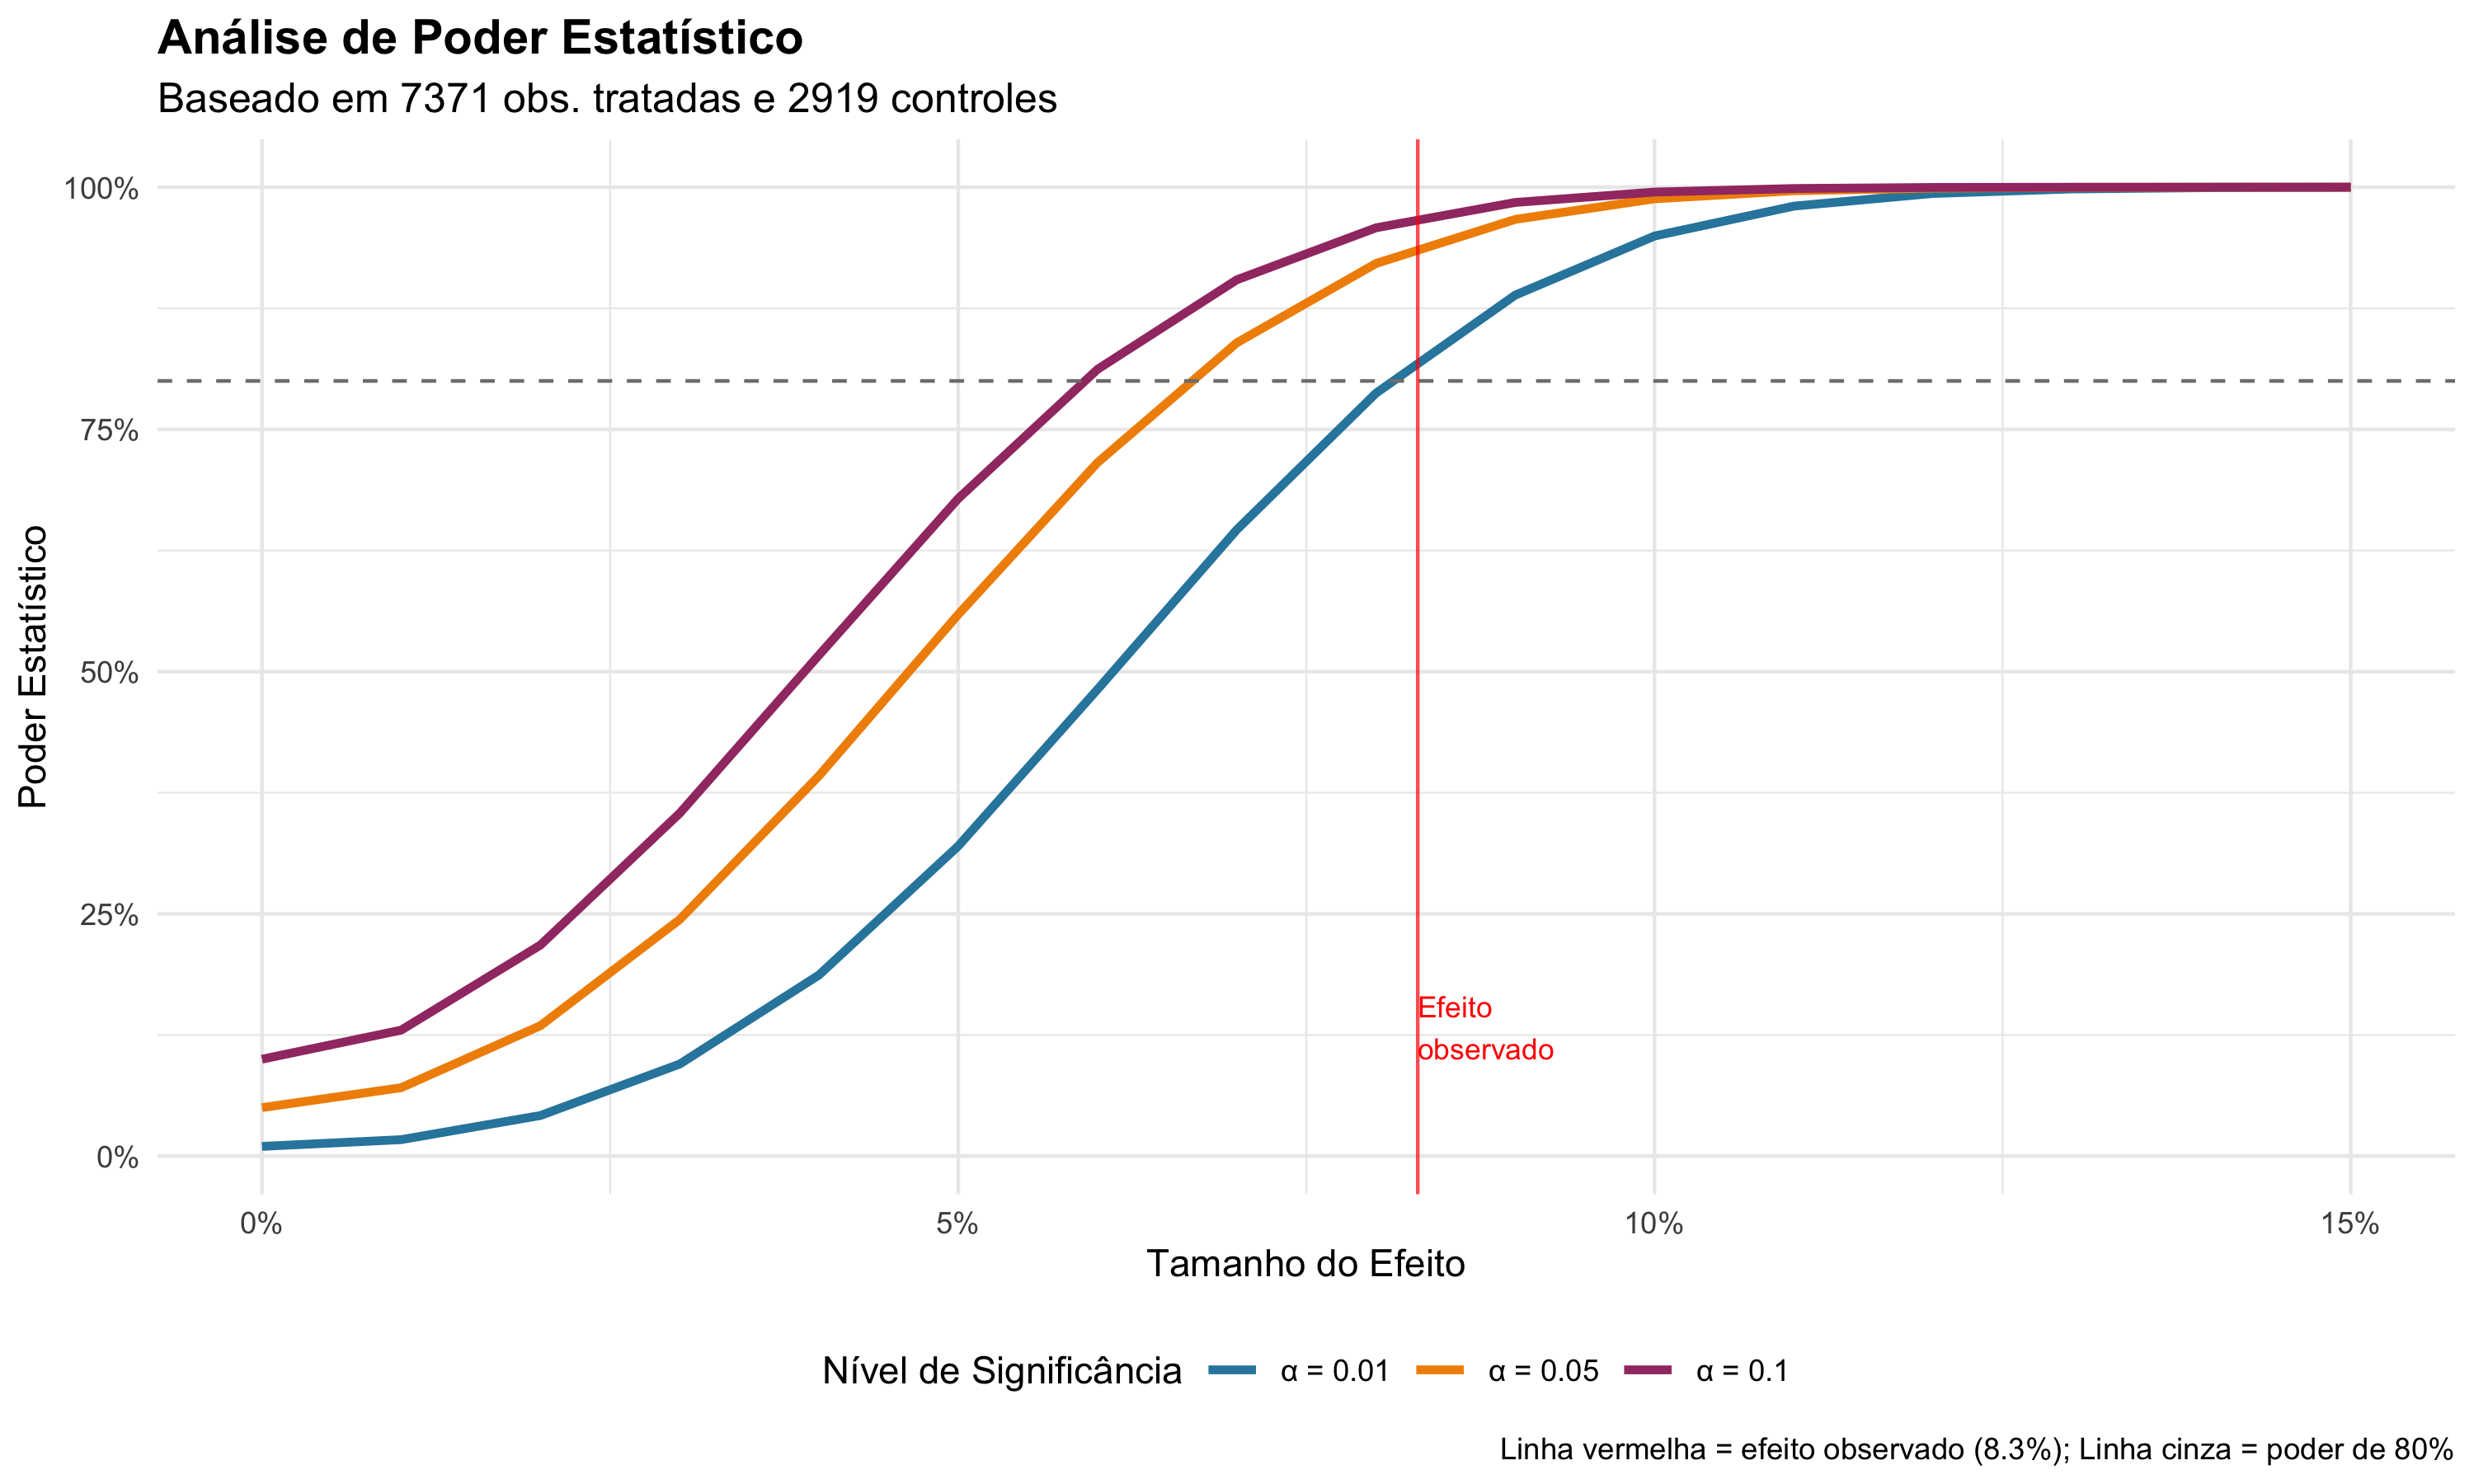
\includegraphics[width=0.7\textwidth]{../../../data/outputs/additional_figures/power_analysis_simulation.png}
\end{figure}

\begin{itemize}
    \item Para efeito de \mainattpct{}: poder de 92,1\% ($\alpha = 0,05$)
    \item Design adequado para detectar efeitos economicamente relevantes
\end{itemize}

\textbf{Fonte:} Seção 3.4.2 (TCC, p. 78)
\end{frame}

\end{document}
